\documentclass[11pt]{article}

\usepackage{url}
\usepackage[letterpaper,margin=1in]{geometry}
\usepackage{times}
\usepackage{graphicx}
\usepackage{algorithm}
\usepackage{algorithmic}
\usepackage{program}
\usepackage{subfig}

\begin{document}

\title{Parallel Association Rule Mining With MapReduce}
\author{Justin DeBrabant \\ debrabant@cs.brown.edu \and Weiyi Liu \\
  wliu@cs.brown.edu}
\date{Final Project - CSCI 2950-u - Fall 2011}
\maketitle

\begin{abstract}
In this paper we propose a parallel method of association rule mining
using MapReduce. Using random partitioning of the dataset, we are able
to mine frequent itemsets in parallel at each reducer. After local
frequent itemset mining, the resulting itemsets can be combined to
produce one set of association rules. We show that our solution scales
both with the size of the data as well as the size of the cluster.  
\end{abstract}

\section{Introduction}
\label{sec:intro}

Advances in the way data is collected has led to a explosion in the
amount of data available for analysis. In many cases, the algorithms
and methods used to analyze that data have proven unable to keep up
with the scale of the data being collected. A prime example of this is
transactional datasets, which consist of a database of transactions,
each of which contain a number of items. A question often asked in
transactional data analysis is what relationships exist between the
items in the datasets. Depending on the context of the data being
mined, these relationships can help make busineess decisions or
discover previouly unknown correlations. For example, consider the
canonical example, a large point-of-sale (POS) system that tracks the
purchases of users across a global chain of supermarkets. Each
transaction would represent a set of items that a shopper purchased on
a given visit to the store. Thus, mining the dataset for associations
would yield a set of items that were frequently bought together. The
store could use this information to better layout their store or the
products on the shelves by placing associated items closer
together. Even beyond that, some stores use these association rules to
print relevant coupons at checkout based on a customers current
purchase. The recent emergence of store loyalty cards that track a
customer's purchases \emph{across} transactions (i.e. across multiple
visits to the store), is testament that the data being collected is
only getting more abundant and complex.

While numerous algorithms exist to mine association rules, we show
that it is infeasible to use these on real-world datasets and propose
that parallel methods are needed. In this project, we propose a
parallel algorithm for mining association rules on MapReduce
\cite{Dean2008}.
 Since it's introduction in 2004, MapReduce has become one
of the most popular parallel execution models and is widely supported
and used. Hadoop , the open-source version of MapReduce, allows users
with commodity clusters to launch massively parallel applications
without worrying about the many distributed computing details that are
necessary to consider in other parallel execution models. By coding a
simple \emph{Map} and \emph{Reduce} function, the system handles all
the communication and scheduling between nodes in the cluster while
also providing fault-tolerance. 

We will now more formally introduce the problem of association rule
mining using Agrawal's original formulation in \cite{Agrawal1}. Let
$\mathcal{I} = \{i_1, i_2, i_3, \ldots, i_n\}$ be a set of binary
attributes called items and $\mathcal{D} = \{\tau_1, \tau_2, \tau_3,
  \ldots, \tau_m\}$ be a database of transactions where $\tau_i \subseteq
\mathcal{I}$. An \emph{association rule} is an implication of the form
$X \rightarrow Y$ where $X,Y \subseteq \mathcal{I}$ and $X \cap Y =
\emptyset$. Each association rule has a \emph{support} and a
\emph{confidence} value. The support, $s$, is defined as the
precentage of rules in $\mathcal{D}$ that contain $X \cup Y$. The
confidence, $c$, is defined as the percentage of transactions in
$\mathcal{D}$ that contain $X$ that also contain $Y$. Confidence and
support are important aspects of association rule mining as they are
used as a measure of quality and allow rules below the thresholds
given to be pruned. 

Given the above definition of an association rule, we can now define
the problem of association rule mining. Given a database
$\mathcal{D}$, a minimum support $minsup$ and a minimum confidence
$minconf$, the goal is to generate all rules of the form $X
\rightarrow Y$ s.t. $c > minconf$ and $s > minsup$. 

There are several important aspects to our algorithm that, to our
knowledge, were unexplored in previous work. For one, we take a
probabilistic approach to rule mining. We randomly partition the
dataset in the Mapper phase and the each Reducer performs frequent
itemset mining (FIM) on its local partition of the data. In short, this
provides an even distribution of data to all nodes and prevents
several Reducers from being tasked with all of the work. The reasons
for this will be discussed in more detail in later sections.


\section{Background}

\subsection{Association Rule Mining}

Association rule mining has been researched extensively since it was
first introduced by Agrawal et al. in \cite{Agrawal1}. Its academic
challenges and real-world applicability has kept it a hot topic for
years. There have been numerous algorithms proposed over the years,
including Apriori \cite{Agrawal1} and FP-growth \cite{Han}. In the
above algorithms, the process of finding frequent association rules is
split into two subtasks, which are summarized as follows:

\begin{enumerate}
\item Frequent Itemset Mining (FIM) - In ths task, the objective is to
  find all itemsets that are \emph{frequent}. An itemset is said to be
  frequent if its support is above the user-supplied \emph{minsup}. 
\item Rule Generation - Given the frequent itemsets from (1), the
  objective here is to generate all \emph{strong} rules, that is,
  rules whose confidence is above the user-supplied \emph{minconf}
  threshold. 
\end{enumerate}

Typically, FIM is the dominant phase from the two above, and as such
has received more research attention. In fact, once frequent itemsets
are generated, any rule generation algorithm can be applied to
generate association rules. Thus, improving FIM alone leads to an
improvement in association rule mining. This is the approach we have
taken in this paper. We have parallelized FIM of the database
$\mathcal{D}$ and then use a standard rule generation algorithm to
compute the rules from the final output of the parallel FIM. 

\subsection{MapReduce} 

MapReduce has emerged as one of the most widely used parallel
computing models due in large part to its inherent fault-tolerance and
simple interface. MapReduce is designed to be a shared-nothing system
and works well in cluster with heterogeneous nodes. A single MapReduce
cycle consists of a Map and Reduce function. The Map takes as input a
set of data files, processes them according to the user's
specifications, and outputs a set of key/value pairs. These
intermediate pairs are mapped to their corresponding Reducer by the
underlying framework with the guarantee that all pairs with the same
key value will end up mapped to the same Reducer. The Reducer then
iterates over its set of values and again does processing according to
user-level code. The Reducer then outputs final key/value pairs that
are written to files on the underlying distributed file system with
one output file per Reducer. 

One important characteristic of a MapReduce job is that the job is
only as fast as its slowest component (i.e. the slowest Mapper or the
slowest Reducer). Because of this, ensuring that no Mapper or Reducer
receives an unproportionally large number of key/value pairs is
essential to system performance. Also, because it is a cluster
environment, all data must go over the network. Because of this, it is
important to minimize the number of intermediate key/value pairs that
are generated by Mappers and sent to Reducers. A key advantage of our
implementation over previous parallel approaches is our guaranteed
load-balancing and minimal network traffic. The details of this are
discussed in later sections.

\begin{figure}
\centering
\begin{tabular}{c | l  c | l c}
$\mathcal{D}$ & Candidate Itemset & support & Association Rule & confidence\\ 
\hline
$\tau_1 = \{i_1, i_2, i_3\}$& $\{i_1\}$&1& $i_2 \rightarrow i_3, c =
1$ & 1\\ 
$\tau_2 = \{i_2, i_3, i_4\}$ &$\{i_4\}$&1& $i_3 \rightarrow i_2, c =
1$ & 1\\ 
&$\{i_1, i_2\}$&1&&\\
&$\{i_1, i_3\}$&1&& \\
&$\{i_2, i_4\}$&1&& \\
&$\{i_3, i_4\}$&1&& \\
& $\{i_1, i_2, i_3\}$&1&& \\
& $\{i_2, i_3, i_4\}$&1&& \\
&$\{i_2, i_4\}$&1&& \\
& $\{i_2\}$&2&& \\ 
&$\{i_3\}$&2&& \\
&$\{i_2,i_3\}$&2&& \\
\end{tabular}
\caption{A simple association rule mining example where $\mathcal{I} =
  \{i_1, i_2, i_3, i_4\}$. The database, $\mathcal{D} = \{\tau_1,
  \tau_2\}$  is being mined with $minconf = .8$ The leftmost column
  shows the transactions in $\mathcal{D}$. The middle column
  shows the candidate itemsets that are generated during frequent
  itemset mining. The rightmost column shows the resulting association
rules and their associated confidence.}
\label{fig:example}
\end{figure}

\section{Related Work}

Much work has been done in association rule mining, but the vast
majority of the algorithms are non-parallel and are meant to be run on
single computer. Because of this, the timing of candidate itemset generation and
communication between the mining steps discussed above are not
important factors. The original and most well-known of the association
rule mining algorithms presented in \cite{Agrawal1} is the Apriori
algorithm. Apriori generates candidate itemsets similar to the example
in \ref{fig:example}. However, the current state-of-the-art in
association rule mining goes to the FP-growth algorithm presented in
\cite{Han}. In FP-growth, candidate itemsets aren't explicitly
generated as in Apriori. However, a structure known as an FP-tree is
constructed as a means to index and extract the frequent itemsets. In
our implementation and experimental evaluation, we use the FP-growth
algorithm. 

There have also been several projects in parallel association rule
mining. Most of them, including \cite{Agrawal1996} and
\cite{Zaki1997}, are meant for a shared-memory system architecture.
However, some recent work has been geared to a shared-nothing
architecture such as a Hadoop cluster (\cite{Li2008},
\cite{Li2011}). \cite{Yang2010}, in particular, is the most similar as
it has the same goal: parallel implementation of association rule
mining on MapReduce. However, their approach varies from ours in where
the main computations are done in the MapReduce model and suffers from
several major drawbacks. Their computation model is simple. The
Mappers perform FIM, generate candidate itemsets and emit key/value
pairs in the form of <frequent itemset, count> to the Reducers, which
then sum all incoming counts and prune those below the minimum support
threshold. This approach is similar to the standard wordcount approach
that is often used as a canonical example for MapReduce: the mapper
emits <word, count> pairs and the Reducer sums them. The difference
here is that the size of the data is actually going to grow during FIM
at the Mapper as there could be potentially many candidate
itemsets. An example of the large number of candidate itemsets
generated can be seen in \ref{fig:example}. Now, after exploding the
amount of data in the Mapper, it must all be sent over the network to
the Reducers. This increased network traffic is clearly an issue and
there is no way to get around it in this approach. For example, if
each Mapper wanted to only send a subset of the candidate itemsets it
mined (the popular ones above a support threshold) it would have no
idea of the support of those itemsets in the other reducers. Because
there is no way for mappers to communicate and determine the global
support for a candidate itemset, each Mapper must emit \emph{all} of
its exponentially many candidate itemsets. The other major drawback in
this approach is the potential for skew in the data being sent to
Reducers. Because each Reducer is summing the support counts of a
certain candidate itemset (probably many of them), the Reducers that
are assigned very popular itemsets (i.e. those that appear in a large
portion of transactions) will be sent significantly more data than
other Reducers. In fact, becasue the candidate itemsets in the Mappers
were not filtered, it is likely that a large number of the candidate
itemsets will have very little occurences in the
transactions. Clearly, having some keys with many key/value pairs and
others with almost none is a recipe for data skew. We argue that this
situation, where certain itemsets are far more popular than others in
the transactions, will be the norm in association rule mining, not
just a theoretical worst case scenario.


\section{Our Implementation}

\begin{figure}
\centering
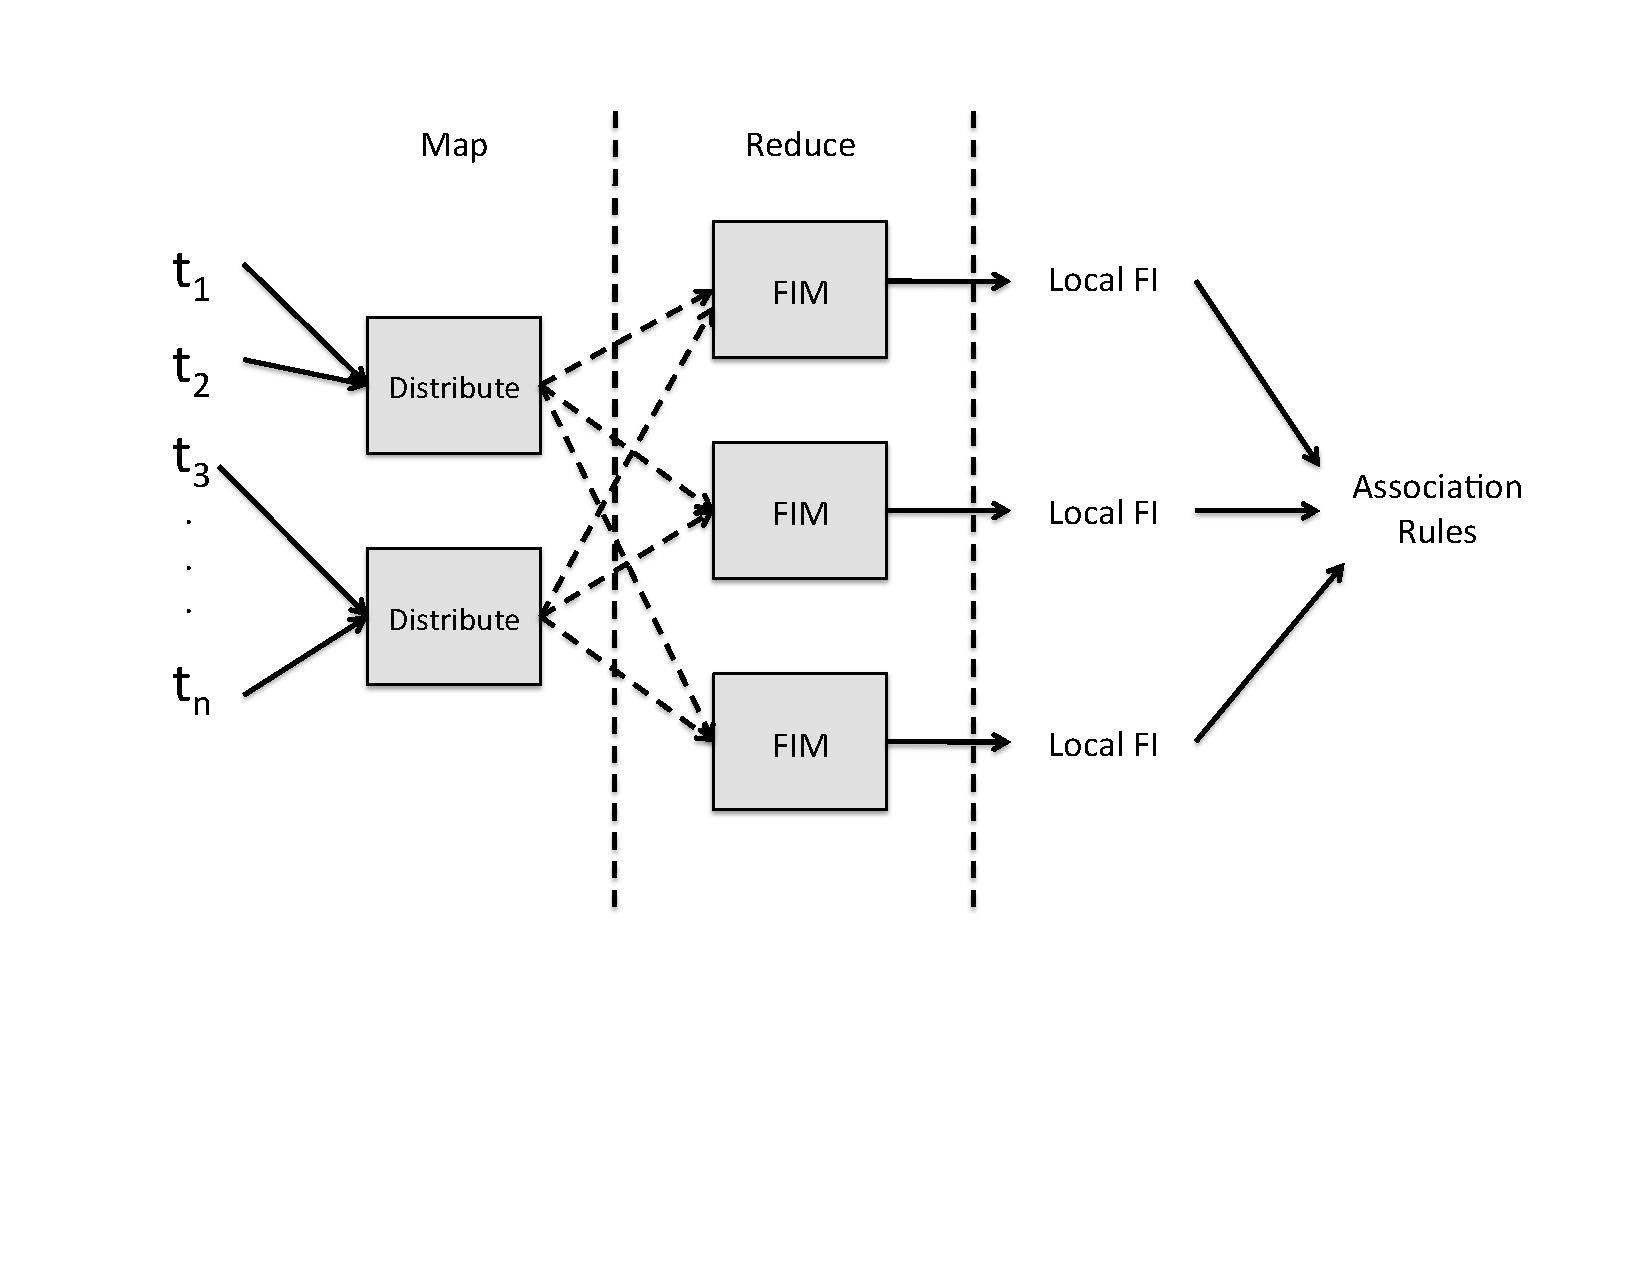
\includegraphics[width=0.7\textwidth]{system_overview}
\caption{A diagram of our implementation.}
\label{fig:overview}
\end{figure}

Our implentation of association rule mining on MapReduce is based on
two key observations. First, that rule mining is dominated by the FIM
stage of the algorithm and that this stage of the algorithm generates
an exponential amount of candidate itemsets with respect to the number
of items in $\mathcal{I}$. To see this, refer to \ref{fig:example},
where a set of 2 transactions with 4 items generates 12 possible
candidate sets. Clearly, with larger data (i.e. more itemsets and
transactions), the cost of generating candidate itemsets will be major
bottleneck in the algorithm. There are ways to make candidate itemset
generation faster. For example, the FP-Growth algorithm uses a FP-tree
to generate and search frequent itemsets, technically never actually
generating all candidate itemsets. The ability of FP-growth to not
generate all candidate itemsets has made it the algorithm of choice
for association rule mining. Unfortunately, the amount of data being
generated (in the form of the FP-trees) is still large and would be
prohibitive to send over the network. Because of this, our algorithm
was designed to avoid sending unfiltered candidate itemsets over the
network as is done in \cite{Yang2010}.

Second, the candidate itemsets generated during FIM are inherently
skewed. That is, several popular itemsets will be in a large number of
the transactions. In \cite{Yang2010}, this will cause skew in the data
as the Reducers that are assigned the most common itemsets will be
sent much more pairs than Reducers that were assigned itemsets that
only appear once or twice (no filtering is done in the candidate
generation phase).

\begin{algorithm}
\caption{Pseudocode for the Map method.}
\label{map}
\begin{algorithmic}
\begin{verbatim}
MAP(key, value)
  int NUM_OUTPUT_GROUPS = 64
  int random_output_group = rand() % NUM_OUTPUT_GROUPS 
  emit(random_output_group, value)
\end{verbatim} 
\end{algorithmic}
\end{algorithm}

\begin{algorithm}
\caption{Pseudocode for the Reduce method.}
\label{reduce}
\begin{algorithmic}
\begin{verbatim}
REDUCE(key, Iterable values)
  out.open("temp.db") 
  for(Text v : values)
     out.write(v)

  List<Itemset> frequent_itemsets = mineFrequentItemsets("temp.db", .02)

  for(Itemset i : frequent_itemsets)
     emit(i.itemset, i.support) 
\end{verbatim} 
\end{algorithmic}
\end{algorithm}

Because of these two considerations, our implementation has pushed the
FIM computation to the Reducer. In the Map phase, each transaction is
sent to a random Reducer group. The number of Reducer groups will
determine the number of transactions that will be in each ``local''
view of the dataset. Essentially, each Reducer is getting a random
sample of the transactions and will perform FIM on its partition of
the data. The pseudocode for Map and Reduce are shown in the figures
for Algorithm 1 and Algorithm 2 respectively. Note, in the pseudocode
we have set the number of map output groups to 64, as this was
empirically verified to be among the ideal range. This is discussed
further in later sections. Also, the function call to mine frequent
itemsets in the Reducer can employ any of the frequent itemset mining
algorithms previously developed. For our experiments, we have chosen
to use FP-growth due to its significant speed advantages over the
other algorithms.

One concern with our parallel method is that it is theoretically
possible for the set of association rules produced with our parallel
method to be different from the set produced in a standard single
machine implementation of association rule mining. To see why, we
first have to understand how frequent itemsets are filtered in
FP-growth. For the FP-growth algorithm, a minimum support is specified
by the user that is used as a minimum threshold which will be used to
filter candidate itemsets. This is usually specified as a decimal
corresponding to the percent of transactions that a given candidate
itemset must be present in order to be included in the set of frequent
itemsets. For example, a value of .2 for $minsup$ would mean that
each candidate itemset would have to be in at least 20\% of the
transactions in order to be considered frequent. The problem arises
when we consider that each Reducer is performing FIM on a subset of
the transactions in the original database. It is possible that at a
given Reducer, a candidate itemset that was frequent in the entire
database would is not frequent at this reducer and thus would be
filtered. This would happen when a Reducer is randomly assigned a
small number of transactions containing the itemset, purely by
chance. Intuitively, this would not be a common case, as most truely
frequent itemsets are present in a very large number of the
transactions. Also, if a given reducer did filter a candidate itemset
that was indeed frequent, that means that a larger than expected
number of the other transactions containing
this itemset were sent to other Reducers, meaning the itemset would be
even \emph{more} likely to be included in the frequent itemsets of
other Reducers. Thus, while a small number of frequent itemsets may be
filtered at a particular Reducer, it is very unlikely that this will
affect the overall confidence of the resulting rule. Of course, we
could always set the local $minsup$ to 0, meaning that each Reducer
shoudl return counts for \emph{all} candidate itemsets in its local
transaction partition. However, this would cause a large increase in
network traffic as well as the runtime of FIM at each local node (the
more candidate itemsets that can be pruned the faster the transactions
can be mined).  Therefore, we have decided to set the local $minsup$
to be the same as the global desired $minsup$. We verify in our
experiments that this has no impact on the set of rules that are
output by comparing it to the set of rules generated in a non-parallel
version of the algorithm. 

\section{Experimental Analysis}

For our experiments, we wanted to test for both correctness and
scalability of our approach. For all experiments, we used Amazon Web
Services to provide the necessary machines. For the non-parallel
testing, we use the Elastic Compute Cloud (EC2). For our parallel
implementation, we used Elastic MapReduce to automatically configure
and launch a dedicated cluster running Hadoop 0.20. For all machines,
on EC2 and Elastic MapReduce, we used the ``m1.xlarge'' instance
type. This instance type has roughly 6.5 EC2 compute units and 17GB of
memory. 

For correctness, we wanted to empirically verify that filtering
itemsets at the local level did not have a significant impact of the
resulting rule set. To do this, we compared several settings of
$minsup$ and verified that the resulting rules and their confidence
values were the same as if we had mined the rules using a non-parallel
version of the algorithm with the same $minsup$. There was little to
report here, as the resulting rule sets were exactly the same in all
cases. We concluded that while theoretically some frequent itemsets
might be filtered at the local level, in practice this would not
happen enough to impact the resulting rule set.

\begin{figure}
\centering
\begin{tabular}{| l | l | l | l | l |}
\hline
& 512MB & 2.5GB & 5GB & 10GB \\
\hline
non-parallel (sec) & 2100 & 29800 & DNF & DNF \\
\hline 
parallel (sec) & 419 & 1943 & 3568 & 6955 \\
\hline
\end{tabular}
\caption{A comparison of runtimes of a sequential FP-growth to our
  parallel implementation. All time are reported in seconds. DNF
  signifies that execution did not finish for that experiment.}
\label{fig:performance}
\end{figure}

For performance, we tested our parallel implentation against a
standard non-parallel version of FP-growth. The table in Figure
\ref{fig:performance} shows the comparison in runtimes between the
non-parallel FP-growth and our parallel MapReduce implementation run
on a 16-node cluster. Note, initial performance gains were quite
modest given that the parallel version was running with 16 times more
computing power. However, as data size was increased, the benefit of
the parallel version became apparent as the non-parallel version was
not able to finish due to memory limitations. The time that the
non-parallel miner ran before running out of memory was also
significant and as datasets became larger it would have quickly become
unfeasible.  

For scalability, we tested both cluster scalability and data
scalability. For cluster scalability, we plotted the results to show
runtimes as well as the relative speedup as more nodes were added to
the cluster. Figure 4(a) shows the results for data scability. It is
interesting to note that our method scaled better than linear. To
explain this, we have to go back to the details of frequent itemset
mining. During the FP-growth algorithm, an FP-tree is made that
represents all possible itemsets from the given set of
transactions. The size of this FP-tree is largely a function of number
of itemsets in the data (assuming all combinations of itemsets are
present in at least 1 of the transactions in the database). Thus,
constructing an FP-tree with $n$ items will cost the same regardless
of the number transactions present. This means that in our datasets where
the number of items is constant but the number of transactions is
increased, there is higher overhead for smaller datasets. This helps
explain the super-linear scaling we see in 4(a). Figure 4(b) and 4(c)
show the results of cluster scalability as functions of runtime and
speedup. Because we kept the data size the same, as the cluster size
was increased each node had a smaller set of transactions but still
the same overhead for constructing the FP-tree (for the same reasons
as discussed above). We believe this is the cause of the suboptimal
speedup we see in 4(c). Because the superoptimal results from 4(a)
and the suboptimal results from 4(c) are related, we believe that if
we had scaled the data and the cluster size up simultaneously, the
resulting curve would have been scaled closer to ideal. Unfortunately,
we didn't the time (or money) left in this project to conduct the
necessary experiments to confim this. 

\section{Conclusions and Future Work}

In this paper, we have presented a parallel implementation of association rule mining
using MapReduce. Our implentation is able to acheive near-linear
speedup and scales to process data sizes that are difficult if not
impossible to acheive using non-parallel techniques on a single
commodity machine. Despite the possibility of our approach giving
incorrect results, we have showed that this is not a problem in
practice. 

As future work, we plan to explore theoretical methods to bound the
uncertainty in our resulting association rules. More formally, we will
be able to guarantee with a probability (1 - $\mathcal{d}$) that the
rules in the result of our parallel implementation will be the exact
same rules that are present in the non-parallel result set. We have
several ideas how to do this, including using a distribution technique
in the Mapper different from partitioning (e.g. various sampling
techniques). 

\begin{figure}
\centering
\subfloat[Data Scability]{\label{fig:data}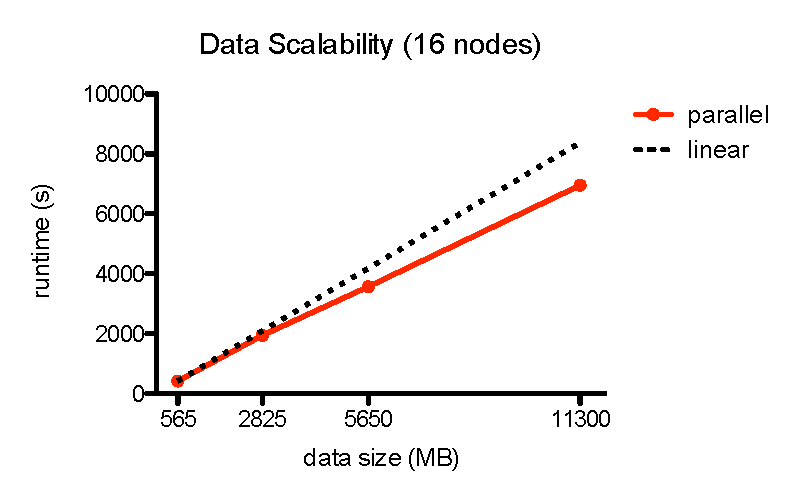
\includegraphics[width=0.33\textwidth]{data_scability}} 
\subfloat[Cluster Scability]{\label{fig:cluster}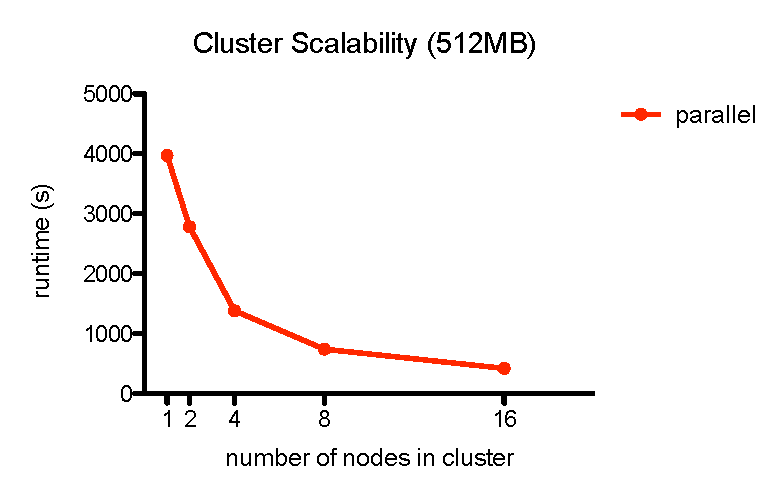
\includegraphics[width=0.33\textwidth]{cluster_scalability}} 
\subfloat[Speedup]{\label{fig:speedup}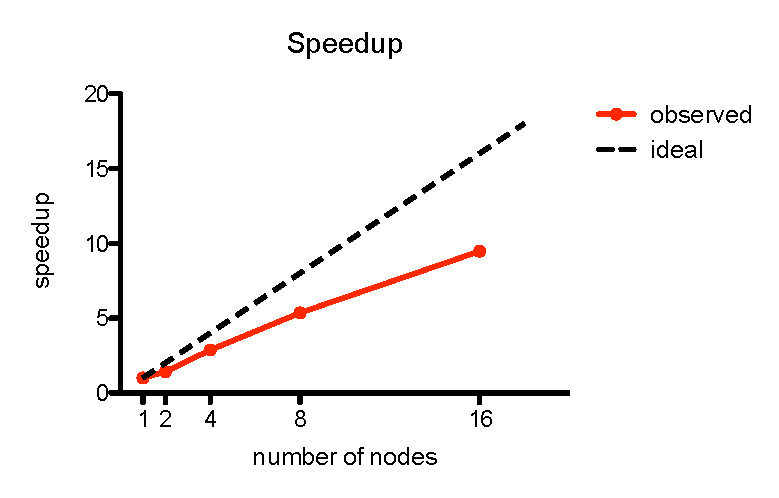
\includegraphics[width=0.33\textwidth]{speedup}} 
\caption{Experimental evaluation of our method. In (a) we show how our
method scales with increased data sizes and a fixed cluster size (16
m1.xlarge nodes). A line corresponding to linear (or ideal)
scalability is plotted alongside. In (b), we show how demonstrate the
performance of our method as cluster size is increased and data size
is held at 512MB. In (c), we show the relative speedup of our method
as we add more nodes to the cluster. An ideal speedup line is plotted
as well. }
\label{fig:experiments}
\end{figure}

\bibliographystyle{plain}
\bibliography{ref}

\end{document}
